\documentclass[20pt]{extarticle}

\usepackage{amsmath, amssymb, amsthm, amsfonts, mathrsfs}
\usepackage{times, flexisym, mdframed, xcolor}
\usepackage{ulem,multicol}
\usepackage{mathtools}
\usepackage{tikz}
\usepackage{hyperref}
\usepackage{graphicx}
\usepackage{bbm}
\usepackage{fancyhdr}
\usepackage{tikz-cd}
\usepackage[doublespacing]{setspace}
\usepackage{pgfplots}
% \usepackage{sectsty}
\setlength{\parindent}{0pt}
\usetikzlibrary{fit, shapes}
\usetikzlibrary{arrows.meta}
\pgfdeclarelayer{background}
\pgfsetlayers{background,main}
\pgfplotsset{compat=1.17}
% \pgfplotsset{soldot/.style={color=black,only marks,mark=*}} \pgfplotsset{holdot/.style={color=black,fill=white,only marks,mark=*}}

\usepackage[paperwidth=400mm,paperheight=300mm,left=10mm,right=150mm, top=10mm, bottom=10mm]{geometry}
\usepackage{draculatheme}
\usepackage[doublespacing]{setspace}

% \sectionfont{\color{draculaorange}}  % sets colour of sections

%Control layout of itemize, enumerate, description (https://ctan.org/pkg/enumitem?lang=en)
\usepackage[shortlabels]{enumitem}
\pagestyle{empty}
\def\endquestion{
  \[\ \]
  \begin{tikzpicture}

    % \foreach \y in {7, 14,...,60}
    % \draw(0,\y mm) -- (80 mm, \y mm);
    % \draw(0,\y mm) -- (170 mm, \y mm);
      \foreach \y in {5, 10,...,60}
          \foreach \x in {5,10,...,170}
          {
              \fill[draculacomment!75] (\x mm,\y mm) circle (.5 pt);
          }
  \end{tikzpicture}
}
\newcommand{\m}{\scalebox{0.5}[1.0]{$-$}}
\newcommand{\LP}{\left(}
\newcommand{\RP}{\right)}
\newcommand{\LS}{\left\lbrace}
\newcommand{\RS}{\right\rbrace}
\newcommand{\LB}{\left[}
\newcommand{\RB}{\right]}
\newcommand{\MM}{\ \middle|\ }

\newcommand{\N}{\mathbb{N}}
\newcommand{\Z}{\mathbb{Z}}
\newcommand{\Q}{\mathbb{Q}}
\newcommand{\R}{\mathbb{R}}
\begin{document}
% \topmargin=-1cm
% \textwidth=170truemm
% \textheight=230truemm

% \begin{large}MATH:1350:XXXX %use your section number
%  \hskip2.7cm{\bf Quiz 1} \hfill{Fall 2021}
% \end{large}
% \vskip0.7cm

% {\bf Name} :

% \hskip1cm ---------------------------------------

% \vskip0.5cm


% --------------------------------------------------------------
%                         Start here
% --------------------------------------------------------------
% \pagestyle{fancy}
% \fancyhf{}
% \rhead{MATH:1005}
% \lhead{Name:\hskip2in ID:}
\noindent
\section*{\textbf{\color{draculaorange}Types of Functions}}
\vskip0.7cm
\subsection*{\textbf{\color{draculaorange}Piecewise Functions}}
\vskip0.7cm
\subsection*{\textbf{\color{draculaorange}Notation}}
\[f(x)=\begin{cases}
  \text{function},&\text{condition}\\
  \vdots&\vdots\\
  \text{function},&\text{condition}\\
\end{cases}\]
\newpage
\subsection*{\textbf{\color{draculared}Example:}}

\begin{tikzpicture}
  \draw[very thin,color=draculacomment] (-0.1,-0.1) grid (17,7);

  \draw[->] (-0.2,0) -- (17,0) node[right] {$t$};
  \draw[->] (0,-0.2) -- (0,7) node[above] {$\Delta  v$};

  \draw[color=draculacyan,domain=0:2]    plot (\x,\x)             node[left] {Stage 1};
  \draw[color=draculayellow,domain=0:4]    plot (\x+2,.5*\x+2)             node[left] {Stage 2};
  \draw[color=draculared,domain=0:3]    plot (\x+6,.6*\x+4)             node[right] {Stage 3};
  \draw[color=draculagreen,domain=0:6]    plot (\x+9,-1*\x+5.8)             node[right] {Falling};
  % \x r means to convert '\x' from degrees to _r_adians:
\end{tikzpicture}

\[f(x)=\begin{cases}
  x,&[0,2)\\
  \frac{1}{2}x,&(2,6]\\
  \frac{3}{5}x,&(6,9]\\
  -x,&(9,15]\\
\end{cases}\]
\subsection*{\textbf{\color{draculared}Example:}}
\begin{tikzpicture}[scale=3]
  \begin{axis} [
    domain=-10:10,
    xmin=-10, xmax=10,
    ymin=-10, ymax=10,
    grid=both,
    % grid style={line width=.08pt, draw=draculacomment!80},
    major grid style={line width=.5pt,draw=draculacomment},
    minor grid style={line width=.08pt,draw=draculacomment!80},
    axis lines=middle,
    minor tick num=4,
    enlargelimits={abs=0.5},
    axis line style={latex-latex},
    ticklabel style={font=\tiny},
]
    \addplot [domain=-10:2,color=draculacyan, smooth, thick] { x};
    \addplot [domain=2:10,color=draculared, smooth, thick] { 2*x};
    \addplot[color=draculacyan,only marks,mark=*] coordinates{(2,2)};
    \addplot[color=draculared,fill=draculabg,only marks,mark=*] coordinates{(2,4)};
  \end{axis}
\end{tikzpicture}
% \begin{tikzpicture}
%   \draw[very thin,color=draculacomment] (-0.1,-0.1) grid (10,10);

%   \draw[->] (-0.2,0) -- (10,0) node[right] {$\ $};
%   \draw[->] (0,-0.2) -- (0,10) node[above] {$\ $};
%   % \addplot[holdot] coordinates{(-2,-2)};
%   % \addplot[soldot] coordinates{(4,1)};
%   \draw[color=draculacyan,domain=0:2]    plot (\x,\x)             ;
%   % \node at (2,2)[circle,fill,color=draculacyan,inner sep=2pt]{};
%   \draw[color=draculayellow,domain=0:8]    plot (\x+2,.5*\x+5);
%   %  node[circle,draw,color=draculayellow] (c) at (2,5){};
%     % \draw[color=draculared,domain=0:3]    plot (\x+6,.6*\x+4)             node[right] {Stage 3};
%   % \draw[color=draculagreen,domain=0:6]    plot (\x+9,-1*\x+5.8)             node[right] {Falling};
%   % \x r means to convert '\x' from degrees to _r_adians:
% \end{tikzpicture}
\newpage
\subsection*{\textbf{\color{draculaorange}Absolute Value}}
\subsection*{\textbf{\color{draculared}Example:}}
\begin{tikzpicture}[scale=3]
  \begin{axis} [
    domain=-10:10,
    xmin=-10, xmax=10,
    ymin=-10, ymax=10,
    grid=both,
    % grid style={line width=.08pt, draw=draculacomment!80},
    major grid style={line width=.5pt,draw=draculacomment},
    minor grid style={line width=.08pt,draw=draculacomment!80},
    axis lines=middle,
    minor tick num=4,
    enlargelimits={abs=0.5},
    axis line style={latex-latex},
    ticklabel style={font=\tiny},
]
\addplot [domain=0:10,color=draculared, smooth, thick] { x};
\addplot [domain=-10:0,color=draculared, smooth, thick] { -x};
\addplot [domain=-10:10,color=draculacyan, smooth, thin] { x};
    % \addplot[color=draculacyan,only marks,mark=*] coordinates{(2,2)};
    % \addplot[color=draculared,fill=draculabg,only marks,mark=*] coordinates{(2,4)};
  \end{axis}
\end{tikzpicture}
\newpage
\subsection*{\textbf{\color{draculared}Example:}}
\begin{tikzpicture}[scale=3]
  \begin{axis} [
    domain=-13:13,
    xmin=-13, xmax=13,
    ymin=-1.5, ymax=1.5,
    grid=both,
    % grid style={line width=.08pt, draw=draculacomment!80},
    major grid style={line width=.5pt,draw=draculacomment},
    minor grid style={line width=.08pt,draw=draculacomment!80},
    axis lines=middle,
    minor tick num=4,
    enlargelimits={abs=0.5},
    axis line style={latex-latex},
    ticklabel style={font=\tiny},
]
\addplot [domain=-13:13,color=draculared,samples=200, smooth, thick] { sin(x r)};
% \addplot [domain=-10:10,color=draculacyan, smooth, thin] { x};
    % \addplot[color=draculacyan,only marks,mark=*] coordinates{(2,2)};
    % \addplot[color=draculared,fill=draculabg,only marks,mark=*] coordinates{(2,4)};
  \end{axis}
\end{tikzpicture}
\newpage
\begin{tikzpicture}[scale=3]
  \begin{axis} [
    domain=-13:13,
    xmin=-13, xmax=13,
    ymin=-1.5, ymax=1.5,
    grid=both,
    % grid style={line width=.08pt, draw=draculacomment!80},
    major grid style={line width=.5pt,draw=draculacomment},
    minor grid style={line width=.08pt,draw=draculacomment!80},
    axis lines=middle,
    minor tick num=4,
    enlargelimits={abs=0.5},
    axis line style={latex-latex},
    ticklabel style={font=\tiny},
]
\addplot [domain=-13:13,color=draculared,samples=200, smooth, thick] { sin(x r)};
\addplot [domain=-13:13,color=draculacyan,samples=800, smooth, thin] { abs(sin(x r))};
% \addplot [domain=-10:10,color=draculacyan, smooth, thin] { x};
    % \addplot[color=draculacyan,only marks,mark=*] coordinates{(2,2)};
    % \addplot[color=draculared,fill=draculabg,only marks,mark=*] coordinates{(2,4)};
  \end{axis}
\end{tikzpicture}
\newpage
\subsection*{\textbf{\color{draculaorange}Even and Odd}}
\vskip0.7cm
\subsection*{\textbf{\color{draculaorange}Definition:}}
A function \(f(x)\) is called:
\begin{itemize}[align=left]
  \item[Even:] {If \(\forall x \in D\) we have \(f(\m x)=f(x)\)}
  \vskip0.7cm
  \item[Odd:] {If \(\forall x \in D\) we have \(f(\m x)=\m f(x)\)}
  \vskip0.7cm
  \item[Neither:] {\(\ \)}
\end{itemize}
\vskip2cm
\subsection*{\textbf{\color{draculaorange}Symmetries:}}
\begin{itemize}[align=left]
  \item[Even:] {\(\ \)}
  \vskip0.7cm
  \item[Odd:] {\(\ \)}
  \vskip0.7cm
  \item[Neither:] {\(\ \)}
\end{itemize}
\newpage
\begin{tikzpicture}[scale=1.3]
  \begin{axis} [
    domain=-10:10,
    xmin=-10, xmax=10,
    ymin=-10, ymax=10,
    grid=both,
    % grid style={line width=.08pt, draw=draculacomment!80},
    major grid style={line width=.5pt,draw=draculacomment},
    minor grid style={line width=.08pt,draw=draculacomment!80},
    axis lines=middle,
    minor tick num=4,
    enlargelimits={abs=0.5},
    % axis line style={latex-latex},
    yticklabels={,,},
    xticklabels={,,}
]
% \addplot [domain=-10:10,color=draculacyan, smooth, thin] { x};
    % \addplot[color=draculacyan,only marks,mark=*] coordinates{(2,2)};
    % \addplot[color=draculared,fill=draculabg,only marks,mark=*] coordinates{(2,4)};
  \end{axis}
\end{tikzpicture}
\vskip0.7cm
\begin{tikzpicture}[scale=1.3]
  \begin{axis} [
    domain=-10:10,
    xmin=-10, xmax=10,
    ymin=-10, ymax=10,
    grid=both,
    % grid style={line width=.08pt, draw=draculacomment!80},
    major grid style={line width=.5pt,draw=draculacomment},
    minor grid style={line width=.08pt,draw=draculacomment!80},
    axis lines=middle,
    minor tick num=4,
    enlargelimits={abs=0.5},
    % axis line style={latex-latex},
    yticklabels={,,},
    xticklabels={,,}
]
% \addplot [domain=-10:10,color=draculacyan, smooth, thin] { x};
    % \addplot[color=draculacyan,only marks,mark=*] coordinates{(2,2)};
    % \addplot[color=draculared,fill=draculabg,only marks,mark=*] coordinates{(2,4)};
  \end{axis}
\end{tikzpicture}
\vskip0.7cm
\begin{tikzpicture}[scale=1.3]
  \begin{axis} [
    domain=-10:10,
    xmin=-10, xmax=10,
    ymin=-10, ymax=10,
    grid=both,
    % grid style={line width=.08pt, draw=draculacomment!80},
    major grid style={line width=.5pt,draw=draculacomment},
    minor grid style={line width=.08pt,draw=draculacomment!80},
    axis lines=middle,
    minor tick num=4,
    enlargelimits={abs=0.5},
    % axis line style={latex-latex},
    yticklabels={,,},
    xticklabels={,,}
]
% \addplot [domain=-10:10,color=draculacyan, smooth, thin] { x};
    % \addplot[color=draculacyan,only marks,mark=*] coordinates{(2,2)};
    % \addplot[color=draculared,fill=draculabg,only marks,mark=*] coordinates{(2,4)};
  \end{axis}
\end{tikzpicture}
\newpage
\newpage
\subsection*{\textbf{\color{draculaorange}Increasing Decreasing}}
\vskip0.7cm
\subsection*{\textbf{\color{draculaorange}Definition:}}
A function \(f(x)\) on an inteval \(I\) is called:
\begin{itemize}[align=left]
  \item[Increasing:] {\(\forall a,b \in I\) if \(a<b\) then \(f(a)<f(b)\)}
  \vskip0.7cm
  \item[Decreasing:] {\(\forall a,b \in I\) if \(a<b\) then \(f(a)>f(b)\)}
\end{itemize}
\begin{tikzpicture}[scale=1.5]
  \begin{axis} [
    domain=-10:10,
    xmin=-10, xmax=10,
    ymin=-10, ymax=10,
    grid=both,
    % grid style={line width=.08pt, draw=draculacomment!80},
    major grid style={line width=.5pt,draw=draculacomment},
    minor grid style={line width=.08pt,draw=draculacomment!80},
    axis lines=middle,
    minor tick num=4,
    enlargelimits={abs=0.5},
    % axis line style={latex-latex},
    yticklabels={,,},
    xticklabels={,,}
]
% \addplot [domain=-10:10,color=draculacyan, smooth, thin] { x};
    % \addplot[color=draculacyan,only marks,mark=*] coordinates{(2,2)};
    % \addplot[color=draculared,fill=draculabg,only marks,mark=*] coordinates{(2,4)};
  \end{axis}
\end{tikzpicture}
\begin{tikzpicture}[scale=1.5]
  \begin{axis} [
    domain=-10:10,
    xmin=-10, xmax=10,
    ymin=-10, ymax=10,
    grid=both,
    % grid style={line width=.08pt, draw=draculacomment!80},
    major grid style={line width=.5pt,draw=draculacomment},
    minor grid style={line width=.08pt,draw=draculacomment!80},
    axis lines=middle,
    minor tick num=4,
    enlargelimits={abs=0.5},
    % axis line style={latex-latex},
    yticklabels={,,},
    xticklabels={,,}
]
% \addplot [domain=-10:10,color=draculacyan, smooth, thin] { x};
    % \addplot[color=draculacyan,only marks,mark=*] coordinates{(2,2)};
    % \addplot[color=draculared,fill=draculabg,only marks,mark=*] coordinates{(2,4)};
  \end{axis}
\end{tikzpicture}
\vskip0.7cm
\newpage
\begin{tikzpicture}[scale=4]
  \begin{axis} [
    domain=-10:10,
    xmin=-10, xmax=10,
    ymin=-10, ymax=10,
    grid=both,
    % grid style={line width=.08pt, draw=draculacomment!80},
    major grid style={line width=.5pt,draw=draculacomment},
    minor grid style={line width=.08pt,draw=draculacomment!80},
    axis lines=middle,
    minor tick num=4,
    enlargelimits={abs=0.5},
    axis line style={latex-latex},
    ticklabel style={font=\tiny},
    % yticklabels={,,},
    % xticklabels={,,}
]
  \addplot [domain=-10:-5,color=draculacyan, smooth, thick] { x};
  \addplot [domain=-5:-2,color=draculagreen, smooth, thick] { (x+5)^2-5};
  \addplot [domain=-2:1,color=draculaorange, smooth, thick] { 4};
  \addplot [domain=1:3,color=draculapink, smooth, thick] { -(x-1)^3+4};
  \addplot [domain=3:4,color=draculapurple, smooth, thick] { (x-3)-4};
  \addplot [domain=4:5,color=draculared, smooth, thick] { -(x-4)-3};
  \addplot [domain=5:10,color=draculayellow, smooth, thick] { (x-5)^2-4};
    % \addplot[color=draculacyan,only marks,mark=*] coordinates{(2,2)};
    % \addplot[color=draculared,fill=draculabg,only marks,mark=*] coordinates{(2,4)};
  \end{axis}
\end{tikzpicture}
\newpage

%   \begin{tikzpicture}[scale=2]
%     \begin{axis} [
%     domain=-10:10,
%     xmin=-10, xmax=10,
%     ymin=-10, ymax=10,
%     grid=both,
%     % grid style={line width=.08pt, draw=draculacomment!80},
%     major grid style={line width=.5pt,draw=draculacomment},
%     minor grid style={line width=.08pt,draw=draculacomment!80},
%     axis lines=middle,
%     minor tick num=4,
%     enlargelimits={abs=0.5},
%     axis line style={latex-latex},
%     ticklabel style={font=\tiny},
%     % yticklabels={,,},
%     % xticklabels={,,}
% ]
%       \addplot [domain=-10:10,color=draculacyan, smooth, thick,<->] { 1 };
%     \end{axis}
%   \end{tikzpicture}
\newpage
\section*{\textbf{\color{draculaorange}"Parent" Functions}}
  \begin{tikzpicture}[scale=2]
    \begin{axis} [
    domain=-10:10,
    xmin=-10, xmax=10,
    ymin=-10, ymax=10,
    grid=both,
    % grid style={line width=.08pt, draw=draculacomment!80},
    major grid style={line width=.5pt,draw=draculacomment},
    minor grid style={line width=.08pt,draw=draculacomment!80},
    axis lines=middle,
    minor tick num=4,
    enlargelimits={abs=0.5},
    axis line style={latex-latex},
    ticklabel style={font=\tiny},
    % yticklabels={,,},
    % xticklabels={,,}
]
      \addplot [domain=-10:10,color=draculacyan, smooth, thick, <->] { x };
    \end{axis}
  \end{tikzpicture}
\begin{tikzpicture}[scale=2]
    \begin{axis} [
    domain=-10:10,
    xmin=-10, xmax=10,
    ymin=-10, ymax=10,
    grid=both,
    % grid style={line width=.08pt, draw=draculacomment!80},
    major grid style={line width=.5pt,draw=draculacomment},
    minor grid style={line width=.08pt,draw=draculacomment!80},
    axis lines=middle,
    minor tick num=4,
    enlargelimits={abs=0.5},
    axis line style={latex-latex},
    ticklabel style={font=\tiny},
    % yticklabels={,,},
    % xticklabels={,,}
]
          \addplot [domain=0:10,color=draculacyan, smooth, thick, ->] { x };
        \addplot [domain=-10:0,color=draculacyan, smooth, thick, <-] { -x };
    \end{axis}
  \end{tikzpicture}


  \begin{tikzpicture}[scale=2]
    \begin{axis} [
    domain=-10:10,
    xmin=-10, xmax=10,
    ymin=-10, ymax=10,
    grid=both,
    % grid style={line width=.08pt, draw=draculacomment!80},
    major grid style={line width=.5pt,draw=draculacomment},
    minor grid style={line width=.08pt,draw=draculacomment!80},
    axis lines=middle,
    minor tick num=4,
    enlargelimits={abs=0.5},
    axis line style={latex-latex},
    ticklabel style={font=\tiny},
    % yticklabels={,,},
    % xticklabels={,,}
]
          \addplot [domain=0:10,color=draculacyan, smooth, samples=200, thick, ->] { sqrt(x) };
    \end{axis}
  \end{tikzpicture}
\begin{tikzpicture}[scale=2]
    \begin{axis} [
    domain=-10:10,
    xmin=-10, xmax=10,
    ymin=-10, ymax=10,
    grid=both,
    % grid style={line width=.08pt, draw=draculacomment!80},
    major grid style={line width=.5pt,draw=draculacomment},
    minor grid style={line width=.08pt,draw=draculacomment!80},
    axis lines=middle,
    minor tick num=4,
    enlargelimits={abs=0.5},
    axis line style={latex-latex},
    ticklabel style={font=\tiny},
    % yticklabels={,,},
    % xticklabels={,,}
]
          \addplot [domain=-10:10,color=draculacyan, smooth, thick, <->] { x^2 };
    \end{axis}
  \end{tikzpicture}
\begin{tikzpicture}[scale=2]
    \begin{axis} [
    domain=-10:10,
    xmin=-10, xmax=10,
    ymin=-10, ymax=10,
    grid=both,
    % grid style={line width=.08pt, draw=draculacomment!80},
    major grid style={line width=.5pt,draw=draculacomment},
    minor grid style={line width=.08pt,draw=draculacomment!80},
    axis lines=middle,
    minor tick num=4,
    enlargelimits={abs=0.5},
    axis line style={latex-latex},
    ticklabel style={font=\tiny},
    % yticklabels={,,},
    % xticklabels={,,}
]
          \addplot [domain=-10:10,color=draculacyan, smooth, thick, <->] { x^3 };
    \end{axis}
  \end{tikzpicture}
\begin{tikzpicture}[scale=2]
    \begin{axis} [
    domain=-10:10,
    xmin=-10, xmax=10,
    ymin=-10, ymax=10,
    grid=both,
    % grid style={line width=.08pt, draw=draculacomment!80},
    major grid style={line width=.5pt,draw=draculacomment},
    minor grid style={line width=.08pt,draw=draculacomment!80},
    axis lines=middle,
    minor tick num=4,
    enlargelimits={abs=0.5},
    axis line style={latex-latex},
    ticklabel style={font=\tiny},
    % yticklabels={,,},
    % xticklabels={,,}
]
      \addplot [domain=0.034:10,color=draculacyan, smooth, samples = 200, thick, <->] { 1/x };
      \addplot [domain=-10:-0.034,color=draculacyan, smooth, samples = 200, thick, <->] { 1/x };
    \end{axis}
  \end{tikzpicture}
\begin{tikzpicture}[scale=2]
    \begin{axis} [
    domain=-10:10,
    xmin=-10, xmax=10,
    ymin=-10, ymax=10,
    grid=both,
    % grid style={line width=.08pt, draw=draculacomment!80},
    major grid style={line width=.5pt,draw=draculacomment},
    minor grid style={line width=.08pt,draw=draculacomment!80},
    axis lines=middle,
    minor tick num=4,
    enlargelimits={abs=0.5},
    axis line style={latex-latex},
    ticklabel style={font=\tiny},
    % yticklabels={,,},
    % xticklabels={,,}
]
      \addplot [domain=0.058:10,color=draculacyan, samples = 200, thick, <->] { 1/(x^2) };
      \addplot [domain=-10:-.058,color=draculacyan, samples = 200, thick, <->] { 1/(x^2) };
    \end{axis}
  \end{tikzpicture}
  \begin{tikzpicture}[scale=2]
    \begin{axis} [
    domain=-5:5,
    xmin=-5, xmax=5,
    ymin=-5, ymax=5,
    grid=both,
    % grid style={line width=.08pt, draw=draculacomment!80},
    major grid style={line width=.5pt,draw=draculacomment},
    minor grid style={line width=.08pt,draw=draculacomment!80},
    axis lines=middle,
    minor tick num=4,
    enlargelimits={abs=0.5},
    axis line style={latex-latex},
    ticklabel style={font=\tiny},
    % yticklabels={,,},
    % xticklabels={,,}
]
      \addplot [domain=-5:5,color=draculacyan, samples = 50, thick, <->] { exp(x) };
    \end{axis}
  \end{tikzpicture}
\newpage
\section*{\textbf{\color{draculaorange}Translation of functions}}
\subsection*{\textbf{\color{draculaorange}Shifts:}}
\begin{itemize}[align=left]
  \item[\underline{\hspace{3cm}}:] {\(f(x)\to f(x-c)\)\\
  \begin{tikzpicture}[scale=1.5]
    \begin{axis} [
      domain=-10:10,
      xmin=-10, xmax=10,
      ymin=-10, ymax=10,
      grid=both,
      % grid style={line width=.08pt, draw=draculacomment!80},
      major grid style={line width=.5pt,draw=draculacomment},
      minor grid style={line width=.08pt,draw=draculacomment!80},
      axis lines=middle,
      minor tick num=4,
      enlargelimits={abs=0.5},
      % axis line style={latex-latex},
      yticklabels={,,},
      xticklabels={,,}
  ]
  \addplot [domain=-10:10,color=draculacyan, smooth, thick] { x^2};
  \addplot [domain=-10:10,color=draculared, smooth, thick] { (x-2)^2};
      % \addplot[color=draculacyan,only marks,mark=*] coordinates{(2,2)};
      % \addplot[color=draculared,fill=draculabg,only marks,mark=*] coordinates{(2,4)};
    \end{axis}
  \end{tikzpicture}}
  \vskip0.7cm
  \item[\underline{\hspace{3cm}}:] {\(f(x)\to f(x+c)\)\\
  \begin{tikzpicture}[scale=1.5]
    \begin{axis} [
      domain=-10:10,
      xmin=-10, xmax=10,
      ymin=-10, ymax=10,
      grid=both,
      % grid style={line width=.08pt, draw=draculacomment!80},
      major grid style={line width=.5pt,draw=draculacomment},
      minor grid style={line width=.08pt,draw=draculacomment!80},
      axis lines=middle,
      minor tick num=4,
      enlargelimits={abs=0.5},
      % axis line style={latex-latex},
      yticklabels={,,},
      xticklabels={,,}
  ]
  \addplot [domain=-10:10,color=draculacyan, smooth, thick] { x^2};
  \addplot [domain=-10:10,color=draculared, smooth, thick] { (x+2)^2};
  % \addplot [domain=-10:10,color=draculacyan, smooth, thick] { x};
      % \addplot[color=draculacyan,only marks,mark=*] coordinates{(2,2)};
      % \addplot[color=draculared,fill=draculabg,only marks,mark=*] coordinates{(2,4)};
    \end{axis}
  \end{tikzpicture}}
  \newpage
  \item[\underline{\hspace{3cm}}:] {\(f(x)\to f(x)-c\)\\
  \begin{tikzpicture}[scale=1.5]
    \begin{axis} [
      domain=-10:10,
      xmin=-10, xmax=10,
      ymin=-10, ymax=10,
      grid=both,
      % grid style={line width=.08pt, draw=draculacomment!80},
      major grid style={line width=.5pt,draw=draculacomment},
      minor grid style={line width=.08pt,draw=draculacomment!80},
      axis lines=middle,
      minor tick num=4,
      enlargelimits={abs=0.5},
      % axis line style={latex-latex},
      yticklabels={,,},
      xticklabels={,,}
  ]
  \addplot [domain=-10:10,color=draculacyan, smooth, thick] { x^2};
  \addplot [domain=-10:10,color=draculared, smooth, thick] { (x)^2-6};
  % \addplot [domain=-10:10,color=draculacyan, smooth, thick] { x};
      % \addplot[color=draculacyan,only marks,mark=*] coordinates{(2,2)};
      % \addplot[color=draculared,fill=draculabg,only marks,mark=*] coordinates{(2,4)};
    \end{axis}
  \end{tikzpicture}}
  \vskip0.7cm
  \item[\underline{\hspace{3cm}}:] {\(f(x)\to f(x)+c\)\\
  \begin{tikzpicture}[scale=1.5]
    \begin{axis} [
      domain=-10:10,
      xmin=-10, xmax=10,
      ymin=-10, ymax=10,
      grid=both,
      % grid style={line width=.08pt, draw=draculacomment!80},
      major grid style={line width=.5pt,draw=draculacomment},
      minor grid style={line width=.08pt,draw=draculacomment!80},
      axis lines=middle,
      minor tick num=4,
      enlargelimits={abs=0.5},
      % axis line style={latex-latex},
      yticklabels={,,},
      xticklabels={,,}
  ]
  \addplot [domain=-10:10,color=draculacyan, smooth, thick] { x^2};
  \addplot [domain=-10:10,color=draculared, smooth, thick] { (x)^2+6};
  % \addplot [domain=-10:10,color=draculacyan, smooth, thick] { x};
      % \addplot[color=draculacyan,only marks,mark=*] coordinates{(2,2)};
      % \addplot[color=draculared,fill=draculabg,only marks,mark=*] coordinates{(2,4)};
    \end{axis}
  \end{tikzpicture}}
\end{itemize}
\newpage
\subsection*{\textbf{\color{draculaorange}Stretching and reflection:}}
For \(1<c\)
\begin{itemize}[align=left]
  \item[\underline{\hspace{3cm}}:] {\(f(x)\to f(cx)\)\\
  \begin{tikzpicture}[scale=1.5]
    \begin{axis} [
      domain=-10:10,
      xmin=-10, xmax=10,
      ymin=-10, ymax=10,
      grid=both,
      % grid style={line width=.08pt, draw=draculacomment!80},
      major grid style={line width=.5pt,draw=draculacomment},
      minor grid style={line width=.08pt,draw=draculacomment!80},
      axis lines=middle,
      minor tick num=4,
      enlargelimits={abs=0.5},
      % axis line style={latex-latex},
      yticklabels={,,},
      xticklabels={,,}
  ]
  \addplot [domain=-10:10,color=draculacyan, smooth, thick] { x^2};
  \addplot [domain=-10:10,color=draculared, smooth, thick] { (3*x)^2};
  % \addplot [domain=-10:10,color=draculacyan, smooth, thick] { x};
      % \addplot[color=draculacyan,only marks,mark=*] coordinates{(2,2)};
      % \addplot[color=draculared,fill=draculabg,only marks,mark=*] coordinates{(2,4)};
    \end{axis}
  \end{tikzpicture}}
  \vskip0.7cm
  \item[\underline{\hspace{3cm}}:] {\(f(x)\to f(\frac{1}{c}x)\)\\
  \begin{tikzpicture}[scale=1.5]
    \begin{axis} [
      domain=-10:10,
      xmin=-10, xmax=10,
      ymin=-10, ymax=10,
      grid=both,
      % grid style={line width=.08pt, draw=draculacomment!80},
      major grid style={line width=.5pt,draw=draculacomment},
      minor grid style={line width=.08pt,draw=draculacomment!80},
      axis lines=middle,
      minor tick num=4,
      enlargelimits={abs=0.5},
      % axis line style={latex-latex},
      yticklabels={,,},
      xticklabels={,,}
  ]

  \addplot [domain=-10:10,color=draculacyan, smooth, thick] { x^2};
  \addplot [domain=-10:10,color=draculared, smooth, thick] { (x/3)^2};
  % \addplot [domain=-10:10,color=draculacyan, smooth, thick] { x};
      % \addplot[color=draculacyan,only marks,mark=*] coordinates{(2,2)};
      % \addplot[color=draculared,fill=draculabg,only marks,mark=*] coordinates{(2,4)};
    \end{axis}
  \end{tikzpicture}}
  \newpage
  \item[\underline{\hspace{3cm}}:] {\(f(x)\to cf(x)\)\\
  \begin{tikzpicture}[scale=1.5]
    \begin{axis} [
      domain=-10:10,
      xmin=-10, xmax=10,
      ymin=-10, ymax=10,
      grid=both,
      % grid style={line width=.08pt, draw=draculacomment!80},
      major grid style={line width=.5pt,draw=draculacomment},
      minor grid style={line width=.08pt,draw=draculacomment!80},
      axis lines=middle,
      minor tick num=4,
      enlargelimits={abs=0.5},
      % axis line style={latex-latex},
      yticklabels={,,},
      xticklabels={,,}
  ]
  \addplot [domain=-10:10,color=draculacyan, smooth, thick] { x^2};
  \addplot [domain=-10:10,color=draculared, smooth, thick] { 6*(x)^2};
  % \addplot [domain=-10:10,color=draculacyan, smooth, thick] { x};
      % \addplot[color=draculacyan,only marks,mark=*] coordinates{(2,2)};
      % \addplot[color=draculared,fill=draculabg,only marks,mark=*] coordinates{(2,4)};
    \end{axis}
  \end{tikzpicture}}
  \vskip0.7cm
  \item[\underline{\hspace{3cm}}:] {\(f(x)\to \frac{1}{c}f(x)\)\\
  \begin{tikzpicture}[scale=1.5]
    \begin{axis} [
      domain=-10:10,
      xmin=-10, xmax=10,
      ymin=-10, ymax=10,
      grid=both,
      % grid style={line width=.08pt, draw=draculacomment!80},
      major grid style={line width=.5pt,draw=draculacomment},
      minor grid style={line width=.08pt,draw=draculacomment!80},
      axis lines=middle,
      minor tick num=4,
      enlargelimits={abs=0.5},
      % axis line style={latex-latex},
      yticklabels={,,},
      xticklabels={,,}
  ]
  \addplot [domain=-10:10,color=draculacyan, smooth, thick] { x^2};
  \addplot [domain=-10:10,color=draculared, smooth, thick] { ((x)^2)/6};
  % \addplot [domain=-10:10,color=draculacyan, smooth, thick] { x};
      % \addplot[color=draculacyan,only marks,mark=*] coordinates{(2,2)};
      % \addplot[color=draculared,fill=draculabg,only marks,mark=*] coordinates{(2,4)};
    \end{axis}
  \end{tikzpicture}}
  \item[\underline{\hspace{3cm}}:] {\(f(x)\to -f(x)\)\\
  \begin{tikzpicture}[scale=1.5]
    \begin{axis} [
      domain=-10:10,
      xmin=-10, xmax=10,
      ymin=-10, ymax=10,
      grid=both,
      % grid style={line width=.08pt, draw=draculacomment!80},
      major grid style={line width=.5pt,draw=draculacomment},
      minor grid style={line width=.08pt,draw=draculacomment!80},
      axis lines=middle,
      minor tick num=4,
      enlargelimits={abs=0.5},
      % axis line style={latex-latex},
      yticklabels={,,},
      xticklabels={,,}
  ]
  \addplot [domain=-10:10,color=draculacyan, smooth, thick] { x^2};
  \addplot [domain=-10:10,color=draculared, smooth, thick] { -(x)^2};
  % \addplot [domain=-10:10,color=draculacyan, smooth, thick] { x};
      % \addplot[color=draculacyan,only marks,mark=*] coordinates{(2,2)};
      % \addplot[color=draculared,fill=draculabg,only marks,mark=*] coordinates{(2,4)};
    \end{axis}
  \end{tikzpicture}}
  \item[\underline{\hspace{3cm}}:] {\(f(x)\to f(-x)\)\\
  \begin{tikzpicture}[scale=1.5]
    \begin{axis} [
      domain=-10:10,
      xmin=-10, xmax=10,
      ymin=-10, ymax=10,
      grid=both,
      % grid style={line width=.08pt, draw=draculacomment!80},
      major grid style={line width=.5pt,draw=draculacomment},
      minor grid style={line width=.08pt,draw=draculacomment!80},
      axis lines=middle,
      minor tick num=4,
      enlargelimits={abs=0.5},
      % axis line style={latex-latex},
      yticklabels={,,},
      xticklabels={,,}
  ]
  \addplot [domain=-10:10,color=draculacyan, smooth, thick] { x^3};
  \addplot [domain=-10:10,color=draculared, smooth, thin] { (-x)^3};
  % \addplot [domain=-10:10,color=draculacyan, smooth, thick] { x};
      % \addplot[color=draculacyan,only marks,mark=*] coordinates{(2,2)};
      % \addplot[color=draculared,fill=draculabg,only marks,mark=*] coordinates{(2,4)};
    \end{axis}
  \end{tikzpicture}}
\end{itemize}

\newpage

\section*{\textbf{\color{draculaorange}Function Arithmetic}}
\begin{itemize}
  \item[]{\(\LP f+g\RP (x)=f(x)+g(x)\)}
  \item[]{\(\LP f-g\RP (x)=f(x)-g(x)\)}
  \item[]{\(\LP f\cdot g\RP (x)=f(x)\cdot g(x)\)}
  \item[]{\(\LP \frac{f}{g}\RP (x)=\frac{f(x)}{g(x)}\)}
\end{itemize}
\subsection*{\textbf{\color{draculared}\textbf{Example:}}}
If we let \(f(x)=x^2\) and \(g(x)=4x^3\)
\begin{itemize}[align=left]
  \item[\(\LP f+g\RP (x)=\)]{\underline{\hspace{5cm}}}
  \item[\(\LP f-g\RP (x)=\)]{\underline{\hspace{5cm}}}
  \item[\(\LP f\cdot g\RP (x)=\)]{\underline{\hspace{5cm}}}
  \item[\(\LP \frac{f}{g}\RP (x)=\)]{\underline{\hspace{5cm}}}
\end{itemize}
\newpage
\subsection*{\textbf{\color{draculaorange}Domain}}
\subsubsection*{\textbf{\color{draculaorange}Addition, multiplication \(+\ -\ \cdot\)}}
The domain of $f+g$, $f-g$, and $f\cdot g$ is the intersection of the domains of $f$ and $g$. In other words, $f+g$, $f-g$, and $f\cdot g$ are defined wherever both $f$ and $g$ are defined.
\vskip6cm
\subsubsection*{\textbf{\color{draculaorange}Division}}
For $\frac{f}{g}$, the domain is the intersection of the domains of $f$ and $g$ excluding $x$ where $g(x)$ is 0.\\
\vskip6cm
\subsection*{\textbf{\color{draculaorange}Range}}
\newpage

\subsection*{\textbf{\color{draculaorange}Function Composition}}
We let \(f(x)\) and \(g(x)\) be two functions with
\textit{\color{draculayellow}"compatable"} domain and codomain
\vskip4cm
the compostion of \(f(x)\) and \(g(x)\) written \[\LP f\circ g\RP(x)\]
is defined to be
\[f\LP g\LP x\RP\RP\]
\begin{center}
  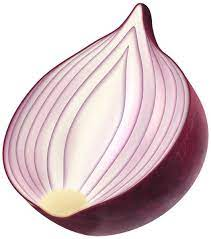
\includegraphics[height=12cm]{onion.jpeg}
\end{center}
\newpage
\subsection*{\textbf{\color{draculared}Example:}}
Let \(f(x)=x^2\) and \(g(x)=\sqrt{x}=\underline{\hspace{2cm}}\)
\vskip4cm
\(\LP f\circ g\RP(x)=\)\\
\vskip8cm
\(\LP g\circ f\RP(x)=\)\\
\newpage
\subsection*{\textbf{\color{draculared}Example:}}
Let \(f(x)=x^2\) and \(g(x)=x+1\)
\vskip4cm
\(\LP f\circ g\RP(x)=\)\\
\vskip8cm
\(\LP g\circ f\RP(x)=\)\\
\newpage

\subsection*{\textbf{\color{draculaorange}Domain}}
The domain of $f\circ g$ is all $x$ in the domain of $g$ so that $g(x)$ is in the domain of $f$.
\vskip8cm


\subsection*{\textbf{\color{draculacyan}Note:}}
The easiest way to find the domain is usually to write an expression for $(f\circ g)(x)$ and find its domain without simplifying.




\newpage

\subsection*{\textbf{\color{draculared}Example:}}
Let \(f:\R\to\R\) where \(f:x\mapsto \frac{1}{x}\), and
\(g:\LP 0,\infty\RP\to \R\) where \(g:x\mapsto x^2\).
\vskip4cm
Find the domain of \(\LP f\circ g\RP(x)\):


\newpage

\subsection*{\textbf{\color{draculacyan}Note:}}
This is one of the most important skills you NEED to have for calculus 1.

\begin{center}
  Easy problems > hard problems
\end{center}
\vskip8cm
further
\begin{center}
  2 Easy problems > a hard problem
\end{center}


\subsection*{\textbf{\color{draculaorange}1:1 (Injective)}}
\vskip 2cm
\begin{center}
  \begin{tikzpicture}[scale=2]


    \filldraw[draculacyan] (-1,0) circle (5pt)            ;
    \filldraw[draculacyan] (-1,1) circle (5pt)            ;
    \filldraw[draculacyan] (-1,2) circle (5pt)            ;
    \filldraw[draculacyan] (-1,3) circle (5pt)            ;
    \filldraw[draculacyan] (-1,4) circle (5pt)            ;
    \filldraw[draculacyan] (-1,5) circle (5pt)            ;
    \filldraw[draculared]  ( 1,0) circle (5pt)            ;
    \filldraw[draculared]  ( 1,1) circle (5pt)            ;
    \filldraw[draculared]  ( 1,2) circle (5pt)            ;
    \filldraw[draculared]  ( 1,3) circle (5pt)            ;
    \filldraw[draculared]  ( 1,4) circle (5pt)            ;
    \filldraw[draculared]  ( 1,5) circle (5pt)            ;
    \filldraw[draculared]  ( 1,6) circle (5pt)            ;
    \filldraw[draculared]  ( 1,7) circle (5pt)            ;

    \draw[-to,ultra thick] (-.75,0) --  node[above] {$f$} (.75,0);
    \draw[-to,ultra thick] (-.75,1) --  node[above] {$f$} (.75,1);
    \draw[-to,ultra thick] (-.75,2) --  node[above] {$f$} (.75,2);
    \draw[-to,ultra thick] (-.75,3) --  node[above] {$f$} (.75,3);
    \draw[-to,ultra thick] (-.75,4) --  node[above] {$f$} (.75,4);
    \draw[-to,ultra thick] (-.75,5) --  node[above] {$f$} (.75,5);

  \end{tikzpicture}
\end{center}

Formally:\\
A function \(f\) is said to be injective if for \(a,b\in D\), with
\(f(a)=f(b)\) then \(a=b\).

\newpage
\subsection*{\textbf{\color{draculaorange}Inverse Functions}}
\vskip 2cm

\begin{center}
  \begin{tikzpicture}[scale=2]


    \filldraw[draculacyan] (-1,0) circle (5pt)            ;
    \filldraw[draculacyan] (-1,1) circle (5pt)            ;
    \filldraw[draculacyan] (-1,2) circle (5pt)            ;
    \filldraw[draculacyan] (-1,3) circle (5pt)            ;
    \filldraw[draculacyan] (-1,4) circle (5pt)            ;
    \filldraw[draculacyan] (-1,5) circle (5pt)            ;
    \filldraw[draculared]  ( 1,0) circle (5pt)            ;
    \filldraw[draculared]  ( 1,1) circle (5pt)            ;
    \filldraw[draculared]  ( 1,2) circle (5pt)            ;
    \filldraw[draculared]  ( 1,3) circle (5pt)            ;
    \filldraw[draculared]  ( 1,4) circle (5pt)            ;
    \filldraw[draculared]  ( 1,5) circle (5pt)            ;
    \filldraw[draculared]  ( 1,6) circle (5pt)            ;
    \filldraw[draculared]  ( 1,7) circle (5pt)            ;

    \draw[to-,ultra thick] (-.75,0) --  node[above] {$f^{\m 1}$} (.75,0);
    \draw[to-,ultra thick] (-.75,1) --  node[above] {$f^{\m 1}$} (.75,1);
    \draw[to-,ultra thick] (-.75,2) --  node[above] {$f^{\m 1}$} (.75,2);
    \draw[to-,ultra thick] (-.75,3) --  node[above] {$f^{\m 1}$} (.75,3);
    \draw[to-,ultra thick] (-.75,4) --  node[above] {$f^{\m 1}$} (.75,4);
    \draw[to-,ultra thick] (-.75,5) --  node[above] {$f^{\m 1}$} (.75,5);

  \end{tikzpicture}


\end{center}
\newpage
\section*{\textbf{\color{draculaorange}Identity Function}}
We the function \(f:D\to D\) with \(x\mapsto x\) the "Identity" function
\[f(x)=x\]
\[id_D(x)=x\]
% \[\mathbbm{1}(x)=x\]
\section*{\textbf{\color{draculaorange}Inverting a function}}
Let \(f:D\to R\) be an injective function. Then \(g:R\to D\) is an inverse of
\(f\) if
\[\LP f\circ g\RP(r)=r\]
and
\[\LP g\circ f\RP(d)=d\]
we write \(g\) as \(f^{\m 1}\).
\newpage
\section*{\textbf{\color{draculaorange}Tests for injectivity}}
Let $f: A \to B$
\begin{itemize}
  \item[I]{Algebraic
        \begin{enumerate}
          \item {Proving something is NOT injective, find a counterexample:\\
                find $x_1, x_2 \in A$ such that $f\left(x_1\right)=f\left(x_2\right)$ BUT $x_1 \neq x_2$}
          \item{Proving something is injective: Find a contradiction:
                \begin{enumerate}
                  \item{Assume $3 x_1, x_2 \in A, x_1 \neq x_2$ but $f\left(x_1\right)=f\left(x_2\right)$}
                  \item{Write $f\left(x_1\right)=f\left(x_0\right)$}
                  \item{Simplify until you find a contradiction.}
                \end{enumerate}
                }
        \end{enumerate}
        }
        \newpage
        \item[II]{Graphical
        \begin{enumerate}
          \item{Horizontal line test
          \begin{enumerate}
            \item{Graph the function}
            \item{Run a Horizontal line across the graph.}
          \end{enumerate}
          }
        \end{enumerate}
        }
\end{itemize}

\begin{tikzpicture}[scale=2]
  \begin{axis} [
        domain=-10:10,
        xmin=-10, xmax=10,
        ymin=-10, ymax=10,
        grid=both,
        % grid style={line width=.08pt, draw=draculacomment!80},
        major grid style={line width=.5pt,draw=draculacomment},
        minor grid style={line width=.08pt,draw=draculacomment!80},
        axis lines=middle,
        minor tick num=4,
        enlargelimits={abs=0.5},
        axis line style={latex-latex},
        ticklabel style={font=\tiny},
        % yticklabels={,,},
        % xticklabels={,,}
    ]
\addplot [domain=-10:10,color=draculacyan,samples=200, smooth, thick] { x^2};
% \addplot [domain=-10:10,color=draculared,samples=200, smooth, thick] { x};
% \addplot [domain=0:10,color=draculacyan, smooth, thin] { x^(1/2)};
    % \addplot[color=draculacyan,only marks,mark=*] coordinates{(2,2)};
    % \addplot[color=draculared,fill=draculabg,only marks,mark=*] coordinates{(2,4)};
  \end{axis}
\end{tikzpicture}
\newpage
\begin{tikzpicture}[scale=2]
  \begin{axis} [
        domain=-10:10,
        xmin=-10, xmax=10,
        ymin=-10, ymax=10,
        grid=both,
        % grid style={line width=.08pt, draw=draculacomment!80},
        major grid style={line width=.5pt,draw=draculacomment},
        minor grid style={line width=.08pt,draw=draculacomment!80},
        axis lines=middle,
        minor tick num=4,
        enlargelimits={abs=0.5},
        axis line style={latex-latex},
        ticklabel style={font=\tiny},
        % yticklabels={,,},
        % xticklabels={,,}
    ]
\addplot [domain=-10:10,color=draculacyan,samples=200, smooth, thick] { 1/3*x^3};
% \addplot [domain=-10:10,color=draculared,samples=200, smooth, thick] { x};
% \addplot [domain=0:10,color=draculacyan, smooth, thin] { x^(1/2)};
    % \addplot[color=draculacyan,only marks,mark=*] coordinates{(2,2)};
    % \addplot[color=draculared,fill=draculabg,only marks,mark=*] coordinates{(2,4)};
  \end{axis}
\end{tikzpicture}

\newpage
\section*{\textbf{\color{draculaorange}Finding an Inverse}}
\begin{enumerate}
  \item{
    Algebraic:
    \begin{enumerate}
      \item{
      Verify \(f\) is injective.
      }
      \item{write \(f(x)\) as \(y\)}
      \item{exchange \(x\) and \(y\)}
      \item{solve for x}
      \item{exchange \(x\) and \(y\)}
      \item{write \(y\) as \(f^{\m 1}\)}
    \end{enumerate}
    \subsection*{\textbf{\color{draculared}Example:}}
    \(f(x)=e^x\)
    \subsection*{\textbf{\color{draculared}Example:}}
    \(f(x)=\frac{x+1}{x-1}\)
    \newpage
  }
  \item{
    Geometric:
    \begin{enumerate}
      \item{Graph \(f\)}
      \item{
      Verify \(f\) is injective.
      }
      \item{Reflect \(f\) across \(id_D\)}
    \end{enumerate}

  }
\end{enumerate}
\subsection*{\textbf{\color{draculared}Example:}}

\begin{tikzpicture}[scale=2]
  \begin{axis} [
        domain=-10:10,
        xmin=-10, xmax=10,
        ymin=-10, ymax=10,
        grid=both,
        % grid style={line width=.08pt, draw=draculacomment!80},
        major grid style={line width=.5pt,draw=draculacomment},
        minor grid style={line width=.08pt,draw=draculacomment!80},
        axis lines=middle,
        minor tick num=4,
        enlargelimits={abs=0.5},
        axis line style={latex-latex},
        ticklabel style={font=\tiny},
        % yticklabels={,,},
        % xticklabels={,,}
    ]
\addplot [domain=-10:10,color=draculacyan,samples=200, smooth, thick] { x^2};
\addplot [domain=-10:10,color=draculared,samples=200, smooth, thin] { x};
% \addplot [domain=0:10,color=draculacyan, smooth, thin] { x^(1/2)};
    % \addplot[color=draculacyan,only marks,mark=*] coordinates{(2,2)};
    % \addplot[color=draculared,fill=draculabg,only marks,mark=*] coordinates{(2,4)};
  \end{axis}
\end{tikzpicture}
\newpage
\subsection*{\textbf{\color{draculared}Example:}}
\begin{tikzpicture}[scale=2]
  \begin{axis} [
        domain=-10:10,
        xmin=-10, xmax=10,
        ymin=-10, ymax=10,
        grid=both,
        % grid style={line width=.08pt, draw=draculacomment!80},
        major grid style={line width=.5pt,draw=draculacomment},
        minor grid style={line width=.08pt,draw=draculacomment!80},
        axis lines=middle,
        minor tick num=4,
        enlargelimits={abs=0.5},
        axis line style={latex-latex},
        ticklabel style={font=\tiny},
        % yticklabels={,,},
        % xticklabels={,,}
    ]
\addplot [domain=-10:10,color=draculacyan,samples=200, smooth, thick] { x^3};
\addplot [domain=-10:10,color=draculared,samples=200, smooth, thin] { x};
% \addplot [domain=0:10,color=draculacyan, smooth, thin] { x^(1/2)};
    % \addplot[color=draculacyan,only marks,mark=*] coordinates{(2,2)};
    % \addplot[color=draculared,fill=draculabg,only marks,mark=*] coordinates{(2,4)};
  \end{axis}
\end{tikzpicture}







\end{document}